\documentclass[
	% -- opções da classe memoir --
	12pt,				% tamanho da fonte
	oneside,			% para impressão em verso e anverso. Oposto a twoside
	a4paper,			% tamanho do papel. 
	% -- opções da classe abntex2 --
	%chapter=TITLE,		% títulos de capítulos convertidos em letras maiúsculas
	%section=TITLE,		% títulos de seções convertidos em letras maiúsculas
	%subsection=TITLE,	% títulos de subseções convertidos em letras maiúsculas
	%subsubsection=TITLE,% títulos de subsubseções convertidos em letras maiúsculas
	% -- opções do pacote babel --
	english,			% idioma adicional para hifenização
	french,				% idioma adicional para hifenização
	spanish,			% idioma adicional para hifenização
	brazil,				% o último idioma é o principal do documento
]{abntex2}


% ---
% PACOTES
% ---

% ---
% Pacotes fundamentais 
% ---
\usepackage{lmodern}			% Usa a fonte Latin Modern
\usepackage[T1]{fontenc}		% Selecao de codigos de fonte.
\usepackage[utf8]{inputenc}		% Codificacao do documento (conversão automática dos acentos)
\usepackage{indentfirst}		% Indenta o primeiro parágrafo de cada seção.
\usepackage{color}				% Controle das cores
\usepackage{graphicx}			% Inclusão de gráficos
\usepackage{microtype} 			% para melhorias de justificação
% ---

% ---
% Pacotes adicionais, usados no anexo do modelo de folha de identificação
% ---
\usepackage{multicol}
\usepackage{multirow}
% ---
	
% ---
% Pacotes adicionais, usados apenas no âmbito do Modelo Canônico do abnteX2
% ---
\usepackage{lipsum}				% para geração de dummy text
% ---
% ---
% PACOTES QUE EU (Álvaro Ferreira Pires de Paiva) ADICIONEI
% ---
\usepackage{float}
\usepackage{longtable}
\usepackage{amsmath}
\usepackage{amsfonts}
\usepackage{listings}
\usepackage{xcolor}
\usepackage{csvsimple}

% C++
\definecolor{verde}{rgb}{0,0.5,0}
\lstset{
  language=C++,
  basicstyle=\ttfamily\small,
  keywordstyle=\color{blue},
  stringstyle=\color{verde},
  commentstyle=\color{red},
  extendedchars=true,
  showspaces=false,
  showstringspaces=false,
  numbers=left,
  numberstyle=\tiny,
  breaklines=true,
  backgroundcolor=\color{green!10},
  breakautoindent=true,
  captionpos=b,
  xleftmargin=0pt,
}

\definecolor{jpurple}{rgb}{0.5,0,0.35}
\lstset{
    language=Python,
    basicstyle=\ttfamily\small,
    keywordstyle=\color{jpurple}\bfseries,
    stringstyle=\color{red},
    commentstyle=\color{verde},
    morecomment=[s][\color{blue}]{/**}{*/},
    extendedchars=true,
    showspaces=false,
    showstringspaces=false,
    numbers=left,
    numberstyle=\tiny,
    breaklines=true,
    backgroundcolor=\color{cyan!10},
    breakautoindent=true,
    captionpos=b,
    xleftmargin=0pt,
    tabsize=2
}

% ---
% Pacotes de citações
% ---
\usepackage[brazilian,hyperpageref]{backref}	 % Paginas com as citações na bibl
\usepackage[alf]{abntex2cite}	% Citações padrão ABNT

% ---
% Configurações do pacote backref
% Usado sem a opção hyperpageref de backref
\renewcommand{\backrefpagesname}{Citado na(s) página(s):~}
% Texto padrão antes do número das páginas
\renewcommand{\backref}{}
% Define os textos da citação
\renewcommand*{\backrefalt}[4]{
	\ifcase #1 %
		Nenhuma citação no texto.%
	\or
		Citado na página #2.%
	\else
		Citado #1 vezes nas páginas #2.%
	\fi}%
% ---

% --- 
% CONFIGURAÇÕES DE PACOTES
% --- 

% ---
% Configurações do pacote backref
% Usado sem a opção hyperpageref de backref
\renewcommand{\backrefpagesname}{Citado na(s) página(s):~}
% Texto padrão antes do número das páginas
\renewcommand{\backref}{}
% ---

% ---
% Configurações de aparência do PDF final

% alterando o aspecto da cor azul
\definecolor{blue}{RGB}{41,5,195}

% informações do PDF
\makeatletter
\hypersetup{
     	%pagebackref=true,
		pdftitle={\@title}, 
		pdfauthor={\@author},
	    pdfcreator={LaTeX with abnTeX2},
		pdfkeywords={abnt}{latex}{abntex}{abntex2}{relatório técnico}, 
		colorlinks=true,       		% false: boxed links; true: colored links
    	linkcolor=blue,          	% color of internal links
    	citecolor=blue,        		% color of links to bibliography
    	filecolor=magenta,      		% color of file links
		urlcolor=blue,
		bookmarksdepth=4
}
% --- 

% --- 
% Espaçamentos entre linhas e parágrafos 
% --- 

% O tamanho do parágrafo é dado por:
\setlength{\parindent}{1.3cm}

% Controle do espaçamento entre um parágrafo e outro:
\setlength{\parskip}{0.2cm}  % tente também \onelineskip

% ---
% compila o indice
% ---
\makeindex
% ---


%----------------------------------------------------------------------------------------
%	TITLE PAGE
%----------------------------------------------------------------------------------------

\newcommand*{\titleGP}{\begingroup % Create the command for including the title page in the document

\begin{flushleft}
\textbf{Instituição:} Universidade Federal do Rio Grande do Norte -- UFRN \\
\textbf{Unidade:} Instituto Metrópole Digital -- IMD \\
\textbf{Curso:} Bacharelado em Tecnologia da Informação -- BTI \\
\textbf{Disciplina:} IMD0029 -- Estrutura De Dados Básicas I -- T01 \\
\textbf{Professor:} Selan Rodrigues Dos Santos \\
\end{flushleft}

\centering % Center all text
\vspace*{\baselineskip} % White space at the top of the page

\rule{\textwidth}{1.6pt}\vspace*{-\baselineskip}\vspace*{2pt} % Thick horizontal line
\rule{\textwidth}{0.4pt}\\[\baselineskip] % Thin horizontal line

{\LARGE Relatório técnico de análise de algoritmos de ordenação
}\\[0.2\baselineskip] % Title

\rule{\textwidth}{0.4pt}\vspace*{-\baselineskip}\vspace{3.2pt} % Thin horizontal line
\rule{\textwidth}{1.6pt}\\[\baselineskip] % Thick horizontal line

\vspace*{2\baselineskip} % Whitespace between location/year and editors
\small{Aluno}

{\large{ÁLVARO FERREIRA PIRES DE PAIVA} -- \texttt{2016039162}
\\ \texttt{alvarofepipa@gmail.com} } % Editor list
% {\itshape The University of California \\ Berkeley\par} % Editor affiliation

\vfill % Whitespace between editor names and publisher logo

{\scshape 2017} \\[0.3\baselineskip] % Year published
{\large Natal - RN}\par % Publisher

\endgroup}


% ----
% Início do documento
% ----
\begin{document}

% Retira espaço extra obsoleto entre as frases.
\frenchspacing 

% ----------------------------------------------------------
% ELEMENTOS PRÉ-TEXTUAIS
% ----------------------------------------------------------
% \pretextual

% ---
% Capa
% ---
\pagestyle{empty} % Removes page numbers
\titleGP % This command includes the title page
\cleardoublepage
% ---

% ---
% inserir lista de ilustrações
% ---
\pdfbookmark[0]{\listfigurename}{lof}
\listoffigures*
\cleardoublepage
% ---

% ---
% inserir lista de tabelas
% ---
\pdfbookmark[0]{\listtablename}{lot}
\listoftables*
\cleardoublepage
% ---

% ---
% inserir o sumario
% ---
\pdfbookmark[0]{\contentsname}{toc}
\tableofcontents*
\cleardoublepage
% ---

% ----------------------------------------------------------
% ELEMENTOS TEXTUAIS
% ----------------------------------------------------------
\textual
\chapter{Introdução}
%
% - Algoritmo
%
Um algoritmo é uma sequência finita de passos/instruções, ordenadas de forma lógica, que permitem resolver um determinado problema ou conjunto de problemas de mesmo tipo. Quando tratamos de algoritmo no meio computacional, podemos dividir em 3 partes:
\begin{enumerate}
	\item Entrada de dados;
	\item Processamento;
	\item Saída dos dados resultantes.
\end{enumerate}

%
% - Arranjos
%
No mundo real, lidamos com diversos tipos de dados e um dos modos que possuímos de armazená-los é através de arranjos. Os arranjos são conjuntos/coleções de elementos de tal forma que esses elementos possam ser identificados por um índice ou chave.

Arranjo $A$ de tamanho $n$:
$$
A = 
\begin{bmatrix}
a_{1}, & a_{2}, & a_{3}, & \dots , & a_{n-1}, & a_{n} 
\end{bmatrix}
$$

Identificando elemento do arranjo:
$$ A[1] = a_{1} $$

%
% - Problema da orndeção de arranjos
%
Em determinados casos, precisamos ordenar esses arranjos para facilitar o processamento realizado posteriormente. Esse problema de ordenação é chamado de \textbf{problema da ordenação de um arranjo sequencial}. Como entrada desse problema, temos um arranjo $[ a_{1}, \dots , a_{n} ]$, com $n \in \mathbb{Z}$ e $n > 0$ e a saída é uma permutação $[ a_{\pi1}, \dots , a_{\pi n} ]$ no qual temos a garantia que $a_{\pi 1} \le a_{\pi 2} \le \dots \le a_{\pi n}$.

O presente relatório analisará um total de 7 algoritmos que resolvam o problema citado anteriormente, sendo eles:
\begin{enumerate}
	\item Insertion sort;
	\item Selection sort;
	\item Bubble sort;
	\item Shell sort;
	\item Quick sort;
	\item Merge sort;
	\item Radix sort (LSD).
\end{enumerate}

Esses algoritmos irão ser análisados em 3 situações:
\begin{enumerate}
	\item Arranjos com elementos aleatórios;
	\item Arranjos com elementos não decrescentes;
	\item Arranjos com elementos não crescentes;
\end{enumerate}
\chapter{Metodologia}
Esse capítulo constará, respectivamente, com as informações técnicas referentes aos experimentos (características do computador utilizado, sistema operacional, linguagem de programação adotada, etc), os algoritmos implementados (uma breve explicação de cada um e seus respectivos códigos) e uma explicação de cada cenário analisado nesse trabalho.

\section{Informações técnicas}
Para a realização do trabalho, foi utilizado um notebook com as seguintes características:

\begin{tabular}{| r | l |}
	\hline
	\textbf{Fabricante}   & Acer \\
	\hline
	\textbf{Modelo}       & Aspire 4739 \\
	\hline
	\textbf{Placa-mãe}    & HMA CP (versão 1.08) \\
	\hline
	\textbf{Disco}        & Hitachi HTS54757 (750 GB) \\
	\hline
	\textbf{RAM}          & 8 GB \\
	\hline
	\textbf{Processador}  & Intel Core i5-480M (2.67GHz) \\
	\hline
	\textbf{Gráficos}     & Intel Ironlake Mobile \\
	\hline
	\textbf{Sistema base} & Ubuntu 16.04.2 LTS 64-bit \\
	\hline
\end{tabular}

A linguagem de programação adotada foi \textbf{C++} (\textit{C mais mais} ou \textit{C plus plus}). C++ foi escolhido devido ser considerado uma linguagem poderosa para a resolução de problemas de baixo e alto nível, prezando pela performance rápida, pois cada recursos presente foi criteriosamente projetado para se usado onde performance for uma exigência crítica \cite{meyers1997cpp}.

O compilador usado foi o \textbf{g++}, compilador integrante da \texttt{gcc}\footnote{Originalmente escrito como compilador para o sistema operacional GNU, a \textit{GNU Compiler Collection} é um conjunto de compiladores de diversas linguagens (C, C++, Fortran, Ada, Go, etc) e é distribuído pela \textit{Free Software Foundation} (FSF). Seu site oficial é: \url{https://gcc.gnu.org/}.}. Para automatizar a compilação, fez-se uso de um arquivo \texttt{Makefile}\footnote{O arquivo Makefile define regras de compilação que serão seguidas no projeto. Ele é interpretado pelo programa \textbf{make}. A página oficial é: \url{https://www.gnu.org/software/make/}.}:

\lstinputlisting{codes/Makefile}

O editor de texto usado para escrever os códigos usados no trabalho foi o \textbf{Sublime text}\footnote{Site oficial: \url{https://www.sublimetext.com/}.}.

Para a medição de tempo, utilizou-se a biblioteca \texttt{std::chrono} do próprio \texttt{C++}, cálculando o tempo em milissegundos.

\section{Algoritmos implementados}
Nessa seção será descrito os algoritmos implementados e análisados, como também será posto seus respectivos códigos usados no projeto. Perceba que todas as funções possuem a mesma assinatura. Isso foi feito para facilitar na implementação dos códigos no projeto.

\subsection{Insertion sort}
O \textit{Insertion sort} funciona da seguinte maneira: você tem como entrada um vetor de elementos, ele irá percorrer índice por índice e a cada iteração pega aquele elemento e o coloca na posição correta, realizando as trocas necessárias com os elementos anteriores para só depois avançar na iteração. Para entender melhor, veja a imagem a seguir:

\begin{figure}[H]
	\centering
	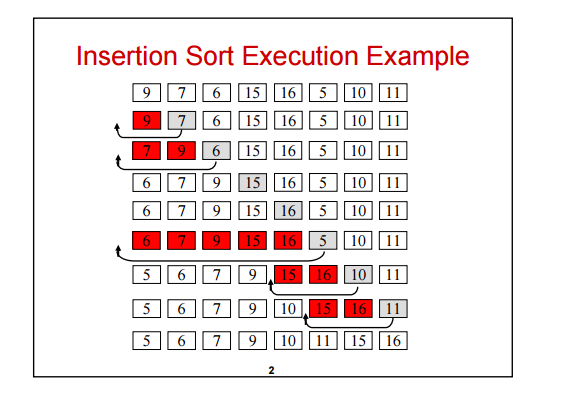
\includegraphics[scale=0.6]{img/insertion-sort.png}
	\caption{Insertion Sort.}
	\small{Imagem retirada de: \url{http://www.geeksforgeeks.org/insertion-sort/}.}
	\label{insertion-sort}
\end{figure}

Ele é considerado um algoritmo estável. Suas informações referentes a complexidade e estabilidade são:

\begin{table}[H]
 \centering
	\begin{tabular}{| r | l |}
		\hline
		\textbf{Complexidade pior caso}   & $O(n^{2})$ \\
		\hline
		\textbf{Complexidade caso médio}  & $O(n^{2})$ \\
		\hline
		\textbf{Complexidade melhor caso} & $O(n)$ \\
		\hline
	\end{tabular}
	\caption{Complexidade do Insertion Sort.}
	\label{t_insertion_sort}
\end{table}

No código a seguir, passamos como argumento o vetor que queremos ordenar. Ignoramos os outros dois parâmetros (\texttt{\_left} e \texttt{\_right}), pois eles foram colocados para apenas termos as mesmas assinaturas que as outras funções do projeto.

\lstinputlisting{codes/insertion_sort.cpp}

\subsection{Selection sort}
O \textit{Selection sort} funciona da seguinte maneira: você tem como entrada um vetor de elementos, ele irá percorrer todo o vetor atrás do menor elemento. Após percorrido, irá trocar a posição do elemento de menor valor com a posição da iteração. Assim, a cada ciclo ele garante que os elementos da posição inicial até $i-1$ ($i$ = iteração) já estejam ordenados. Para entender melhor, veja a imagem a seguir:

\begin{figure}[H]
	\centering
	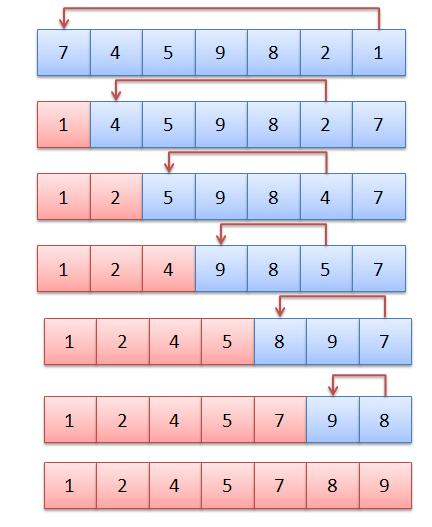
\includegraphics[scale=0.5]{img/selection-sort.jpg}
	\caption{Selection Sort.}
	\small{Imagem retirada de: \url{http://nerds-attack.blogspot.com.br/2012/09/estrutura-dados-selection-sort.html}.}
	\label{selection-sort}
\end{figure}

Suas informações referentes a complexidade são:

\begin{table}[H]
 \centering
	\begin{tabular}{| r | l |}
		\hline
		\textbf{Complexidade pior caso}   & $O(n^{2})$ \\
		\hline
		\textbf{Complexidade caso médio}  & $O(n^{2})$ \\
		\hline
		\textbf{Complexidade melhor caso} & $O(n^{2})$ \\
		\hline
	\end{tabular}
	\caption{Complexidade do Selection Sort.}
	\label{t_selection_sort}
\end{table}

No código a seguir, passamos como argumento o vetor que queremos ordenar. Ignoramos os outros dois parâmetros (\texttt{\_left} e \texttt{\_right}), pois eles foram colocados para apenas termos as mesmas assinaturas que as outras funções do projeto.

\lstinputlisting{codes/selection_sort.cpp}

\subsection{Bubble sort}
O \textit{Bubble sort} funciona da seguinte maneira: você tem como entrada um vetor de elementos, a cada iteração ele irá realizar trocas do elemento atual com os seus seguintes até encontrar a posição ideal do elemento. Para entender melhor, veja a imagem a seguir:

\begin{figure}[H]
	\centering
	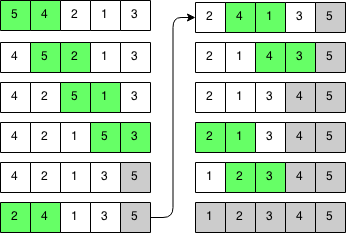
\includegraphics[scale=0.6]{img/bubble-sort.png}
	\caption{Bubble Sort.}
	\small{Imagem retirada de: \url{http://www.coisadeprogramador.com.br/algoritmos-ordenacao-bubble-sort/}.}
	\label{bubble-sort}
\end{figure}

Suas informações referentes a complexidade são:

\begin{table}[H]
 \centering
	\begin{tabular}{| r | l |}
		\hline
		\textbf{Complexidade pior caso}   & $O(n^{2})$ \\
		\hline
		\textbf{Complexidade caso médio}  & $O(n^{2})$ \\
		\hline
		\textbf{Complexidade melhor caso} & $O(n)$ \\
		\hline
	\end{tabular}
	\caption{Complexidade do Bubble Sort.}
	\label{t_bubble_sort}
\end{table}

No código a seguir, passamos como argumento o vetor que queremos ordenar. Ignoramos os outros dois parâmetros (\texttt{\_left} e \texttt{\_right}), pois eles foram colocados para apenas termos as mesmas assinaturas que as outras funções do projeto.

\lstinputlisting{codes/bubble_sort.cpp}

\subsection{Shell sort}
O \textit{Shell sort} é uma extensão do algoritmo \textit{Insertion sort}. Diferente do \textit{Selection sort} que só permite realizar trocas de elementos adjacentes, o \textit{Shell sort} permite trocas de elementos distantes um do outro. Ele funciona da seguinte maneira: você tem como entrada um vetor de elementos, usamos o tamanho desse vetor para decidir qual será a distância inicial entre os elementos que serão trocados. Após cada iteração, dividiremos a distância e assim sucessivamente até atingirmos a troca de elementos adjacentes. Para entender melhor, veja a imagem a seguir:

\begin{figure}[H]
	\centering
	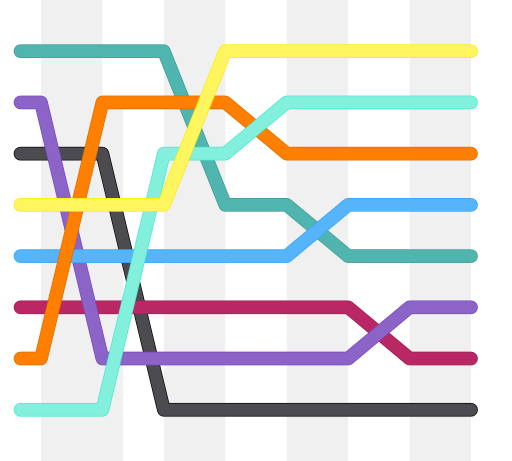
\includegraphics[scale=0.4]{img/shell-sort.png}
	\caption{Shell Sort.}
	\small{Imagem retirada de: \url{https://pt.wikipedia.org/wiki/Shell_sort}.}
	\label{shell-sort}
\end{figure}

A sua análise contêm alguns problemas matemáticos muito difíceis, por causa disso, a sua complexidade ainda não é totalmente conhecida. Suas informações referentes a complexidade até então conhecidas são:

\begin{table}[H]
 \centering
	\begin{tabular}{| r | l |}
		\hline
		\textbf{Complexidade pior caso}   & $O(nlog_{2}n)$ (melhor conhecida) \\
		\hline
		\textbf{Complexidade caso médio}  & depende da sequência da distância \\
		\hline
		\textbf{Complexidade melhor caso} & $O(n)$ \\
		\hline
	\end{tabular}
	\caption{Complexidade do Shell Sort.}
	\label{t_shell_sort}
\end{table}

No código a seguir, passamos como argumento o vetor que queremos ordenar. Ignoramos os outros dois parâmetros (\texttt{\_left} e \texttt{\_right}), pois eles foram colocados para apenas termos as mesmas assinaturas que as outras funções do projeto. Perceba que dividimos a variável `gap' em $2.2$, isso ocorre porque se a divisão der, por exemplo, $2.72727$, pegaremos apenas o valor inteiro, ou seja: $2$. Assim não teremos problemas na execução do algoritmo.

\lstinputlisting{codes/shell_sort.cpp}

\subsection{Quicksort}
O \textit{Quicksort} funciona da seguinte maneira: você tem como entrada um vetor de elementos, é então decidido um pivô e esse pivô irá dividir o vetor em duas partes (uma com números menores que ele na esquerda e outro com números maiores que ele na direita). A cada iteração, iremos aplicar essa mecânica do pivô nos subvetores, gerando outros subvetores até não conseguirmos mais gerar subvetores (vetores de 1 elemento só). Devido a essa mecânica do pivô, teremos os elementos dos subvetores organizados, logo todo o vetor original também estará organizado. Para entender melhor, veja a imagem a seguir:

\begin{figure}[H]
	\centering
	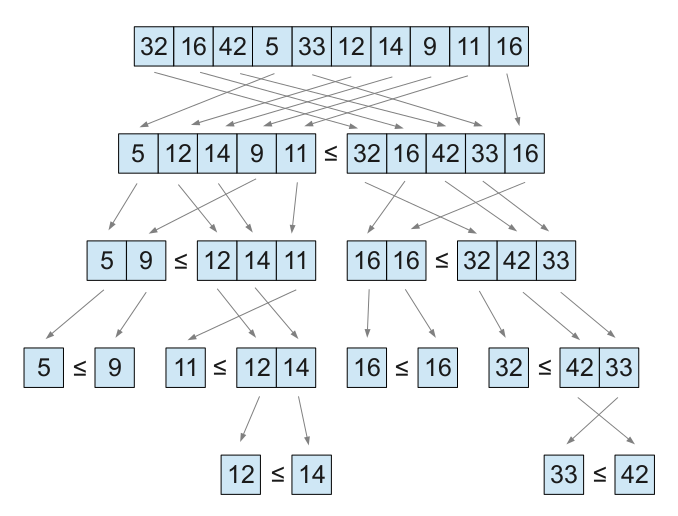
\includegraphics[scale=0.4]{img/quicksort.png}
	\caption{Quicksort.}
	\small{Imagem retirada de: \url{https://simpledevcode.wordpress.com/2014/06/13/quicksort-in-c/}.}
	\label{quicksort}
\end{figure}

Ele é considerado um algoritmo não estável. Suas informações referentes a complexidade são:

\begin{table}[H]
 \centering
	\begin{tabular}{| r | l |}
		\hline
		\textbf{Complexidade pior caso}   & $O(n^{2})$ \\
		\hline
		\textbf{Complexidade caso médio}  & $O(nlogn)$ \\
		\hline
		\textbf{Complexidade melhor caso} & $O(nlogn)$ \\
		\hline
	\end{tabular}
	\caption{Complexidade do Quicksort.}
	\label{t_quicksort}
\end{table}

No código a seguir, passamos como argumento o vetor que queremos ordenar e o índice inicial e final do vetor (respectivamente \texttt{\_left} e \texttt{\_right}). Como esse algoritmo é recursivo\footnote{Recursividade significa que uma sub-rotina (função ou método) que chama a si mesma até atingir uma condição para se encerrar.}, usamos o valor $-1$ no \texttt{\_right} para identificar sua primeira chamada.

\lstinputlisting{codes/quicksort.cpp}

\subsection{Merge sort}
O \textit{Merge sort} funciona da seguinte maneira: você tem como entrada um vetor de elementos, pegamos o indice do meio do vetor e usaremos ele para dividirmos o vetor em duas partes e usarmos o método do \textit{Merge sort} neles, até termos vetores de apenas um elemento. Nisso, iremos aplicar a função \textit{merge} do método e juntaremos esses subvetores formados pelas partes do vetor original. Para entender melhor, veja a imagem a seguir:

\begin{figure}[H]
	\centering
	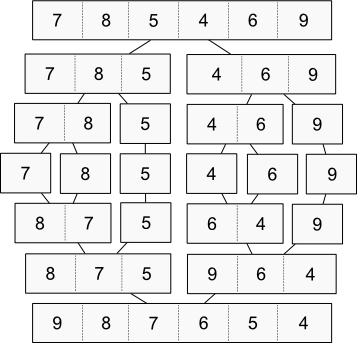
\includegraphics[scale=0.4]{img/merge_sort.png}
	\caption{Merge Sort.}
	\small{Imagem retirada de: \url{https://www.programming-algorithms.net/article/39650/Merge-sort}.}
	\label{merge_sort}
\end{figure}

Suas informações referentes a complexidade são:

\begin{table}[H]
 \centering
	\begin{tabular}{| r | l |}
		\hline
		\textbf{Complexidade pior caso}   & $\theta(nlogn)$ \\
		\hline
		\textbf{Complexidade caso médio}  & $\theta(nlogn)$ \\
		\hline
		\textbf{Complexidade melhor caso} & $\theta(nlogn)$ \\
		\hline
	\end{tabular}
	\caption{Complexidade do Merge Sort.}
	\label{t_merge_sort}
\end{table}

No código a seguir, passamos como argumento o vetor que queremos ordenar e o índice inicial e final do vetor (respectivamente \texttt{\_left} e \texttt{\_right}). Como esse algoritmo é recursivo, usamos o valor $-1$ no \texttt{\_right} para identificar sua primeira chamada. A função \textit{merge} é o que realizará a junção dos dois subvetores.

\lstinputlisting{codes/merge_sort.cpp}

\subsection{Radix sort (LSD)}
O \textit{Radix sort} funciona da seguinte maneira: você tem como entrada um vetor de elementos, a cada iteração ele irá analisar o digito do elemento, podendo começar da esquerda para a direita (\textit{MSD} - \textit{Most significant digit}, digito mais significativo) ou da direita para a esquerda (\textit{LSD} - \textit{Least significant digit}, digito menos significativo), avançando de digito a cada iteração. Para entender melhor, veja a imagem a seguir:

\begin{figure}[H]
	\centering
	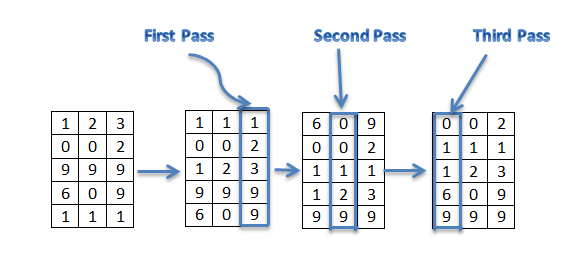
\includegraphics[scale=0.6]{img/radix_sort.png}
	\caption{Radix Sort.}
	\small{Imagem retirada de: \url{http://scanftree.com/Data_Structure/radix-sort}.}
	\label{radix-sort}
\end{figure}

Para todos os casos, ele possuirá o mesmo grau de complexidade. Suas informações referentes a complexidade são:

\begin{table}[H]
 \centering
	\begin{tabular}{| r | l |}
		\hline
		\textbf{Complexidade pior caso}   & $\theta(nk)$ \\
		\hline
		\textbf{Complexidade caso médio}  & \\
		\hline
		\textbf{Complexidade melhor caso} & \\
		\hline
	\end{tabular}
	\caption{Complexidade do Radix Sort.}
	\label{t_radix_sort}
\end{table}

No código a seguir, passamos como argumento o vetor que queremos ordenar. Ignoramos os outros dois parâmetros (\texttt{\_left} e \texttt{\_right}), pois eles foram colocados para apenas termos as mesmas assinaturas que as outras funções do projeto.

\lstinputlisting{codes/radix_sort.cpp}

\subsection{Visão geral}
A tabela a seguire, serve para se ter uma melhor visão dos graus de complexidade de cada algoritmo implementado aqui nesse trabalho.

\begin{table}[H]
 \centering
	\begin{tabular}{| r | p{2.5cm} | p{2.5cm} | p{2.5cm} |}
		\hline
		\multirow{2}{*}{textbf{Algoritmo}} & \multicolumn{3}{c|}{\textbf{Complexidade}} \\
		 & Melhor caso   & Caso médio & Pior caso \\
		\hline
		Insertion sort   & $O(n)$          & $O(n^{2})$                        & $O(n^{2})$ \\
		\hline
		Selection sort   & $O(n^{2})$      & $O(n^{2})$                        & $O(n^{2})$ \\
		\hline
		Bubble sort      & $O(n)$          & $O(n^{2})$                        & $O(n^{2})$ \\
		\hline
		Shell sort       & $O(n)$          & Depende da sequência da distância & $O(nlog_{2}n)$ (melhor conhecida) \\
		\hline
		Quicksort        & $O(nlogn)$      & $O(nlogn)$                        & $O(n^{2})$ \\
		\hline
		Merge sort       & $\theta(nlogn)$ & $\theta(nlogn)$                   & $\theta(nlogn)$ \\
		\hline
		Radix sort (LSD) &                 &                                   & $\theta(nk)$ \\
		\hline
	\end{tabular}
	\caption{Visão geral dos algoritmos de ordenação}
	\label{t_visao_geral}
\end{table}

\section{Cenários}
Foi implementado um total de 3 cenários distintos, nos quais foram aplicados os algoritmos anteriormente apresentados. Os cenários foram:

\begin{enumerate}
	\item Arranjos com elementos aleatórios;
	\item Arranjos com elementos em ordem crescente;
	\item Arranjos com elementos em ordem decrescente.
\end{enumerate}

Em todos os 3 cenários pode ocorrer de haver elementos repetidos. Eles foram aplicados nessa mesma ordem apresentada anteriormente. O mesmo arranjo é usado nos 3 cenários, pois no primeiro ele finaliza com o arranjo ordenado em ordem crescente, aí então é aplicado no segundo cenário e, após, é apenas invertido sua ordem, se tornando em um arranjo decrescente.

Para garantirmos que os cenários não se repitam durante o experimento (os números aleatórios resultarem em um arranjo crescente, por exemplo), foi escrito duas funções, uma para gerar os números aleatórios no arranjo (\texttt{new\_numbers}) e outra para validar o arranjo (\texttt{verify\_order}). O código de ambas se encontra a seguir:

\lstinputlisting{codes/arranjos.cpp}

\section{Geração de gráficos}
Foram executados 50 vezes cada um dos 3 cenários aplicando cada uma das 7 funções para cada uma das 38 entrada, totalizando 39900 registros em um arquivo \textit{CSV}\footnote{\textit{Comma-separated values}. Arquivos de texto em formato de tabela (com linhas e cada atributo na linha é separado de outro atributo por um caractere especial, normalmente ``,'' ou ``;'') usado para armazenamento de dados.}. Precisava-se, então, de gerar uma média de cada um dos cenários, em cada uma das funções e em cada uma das entradas. Para isso, utilizou-se a linguagem \texttt{Python} com a biblioteca \texttt{pandas}, os códigos foram executados no \textit{framework} \texttt{Anaconda} em um \texttt{Jupyter notebook}. O código para gerar um novo \textit{CSV} com as médias dos casos foi:

\lstinputlisting{codes/gerar_csv.py}

Foi utilizado a biblioteca \texttt{bokeh} para gerar os gráficos. Foi atribuido as seguintes cores para cada algoritmo nos gráficos:

\begin{table}[H]
 \centering
	\begin{tabular}{| r | l |}
		\hline
		\textbf{Algoritmo} & \textbf{Cor} \\
		\hline
		Insertion Sort   & Azul \\
		\hline
		Selection Sort   & Verde \\
		\hline
		Bubble Sort      & Laranja \\
		\hline
		Shell Sort       & Vermelho \\
		\hline
		Quicksort        & Roxo \\
		\hline
		Merge Sort       & Marrom \\
		\hline
		Radix sort (LSD) & Preto \\
		\hline
	\end{tabular}
	\caption{Algoritmos e suas respectivas cores nos gráficos.}
	\label{t_graph_color}
\end{table}
\chapter{Resultados}
Nessa capítulo, constará os gráficos e tabelas referentes aos resultados do experimento. Primeiro será apresentado os dados de cada um dos algoritmos e após uma visão geral.

\section{Resultados de cada algoritmo}
A seguir, poderá ser encontrado as tabelas e gráficos referentes as médias finais de cada algoritmo para sua respectiva entrada de elementos. O tempo foi medido em milissegundos. A primeira coluna consta a quantidade de elementos presente no arranjo, as outras 3 colunas constam, respectivamente, o tempo médio que o algoritmo levou para arranjos aleatórios, arranjos com elementos em ordem crescente e arranjos com elementos em ordem decrescente.

Em uma visão geral, podemos notar que os algoritmos realmente agem melhor nos arranjos ordenados crescentemente e que seus piores casos são quando o arranjo está ordenado em ordem decrescente.

\subsection{Insertion sort}
\begin{longtable}{|r|c|c|c|}
	\hline
	\csvreader[
		column count=5,
		no head,
		table head=\hline,
		late after line=\\\hline
	]{csvs/Insertion_Sort.csv}{
		1=\n-elementos, 2=\aleatorio, 3=\crescente, 4=\decrescente
	}{ \n-elementos & \aleatorio & \crescente & \decrescente }
	\caption{Média de tempo do Insertion Sort}
	\label{t-insertion}
\end{longtable}

\begin{figure}[H]
	\centering
	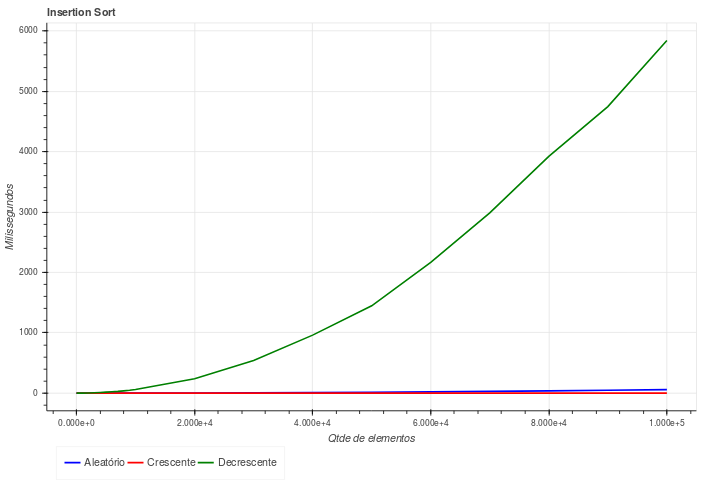
\includegraphics[scale=0.6]{img/algoritmos/insertion_sort.png}
	\caption{Insertion Sort, gráfico de resultados.}
	\label{graph-insertion}
\end{figure}

\subsection{Selection sort}
\begin{longtable}{|r|c|c|c|}
	\hline
	\csvreader[
		column count=5,
		no head,
		table head=\hline,
		late after line=\\\hline
	]{csvs/Selection_Sort.csv}{
		1=\n-elementos, 2=\aleatorio, 3=\crescente, 4=\decrescente
	}{ \n-elementos & \aleatorio & \crescente & \decrescente }
	\caption{Média de tempo do Selection Sort}
	\label{t-selection}
\end{longtable}

\begin{figure}[H]
	\centering
	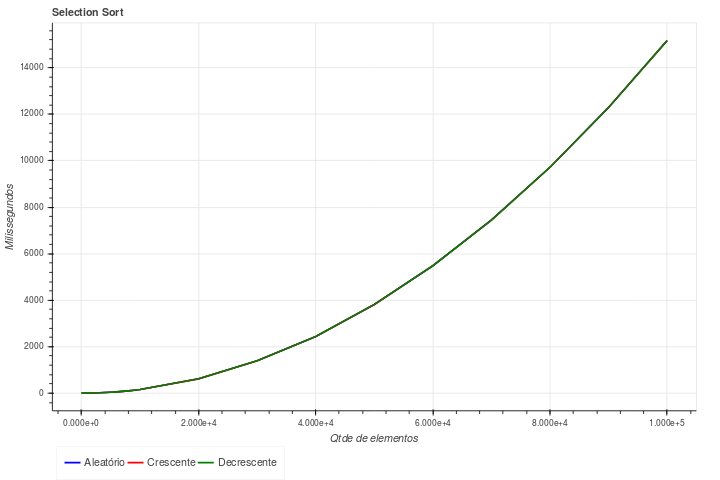
\includegraphics[scale=0.6]{img/algoritmos/selection_sort.png}
	\caption{Selection Sort, gráfico de resultados.}
	\label{graph-selection}
\end{figure}

\subsection{Bubble sort}
\begin{longtable}{|r|c|c|c|}
	\hline
	\csvreader[
		column count=5,
		no head,
		table head=\hline,
		late after line=\\\hline
	]{csvs/Bubble_Sort.csv}{
		1=\n-elementos, 2=\aleatorio, 3=\crescente, 4=\decrescente
	}{ \n-elementos & \aleatorio & \crescente & \decrescente }
	\caption{Média de tempo do Bubble Sort}
	\label{t-bubble}
\end{longtable}

\begin{figure}[H]
	\centering
	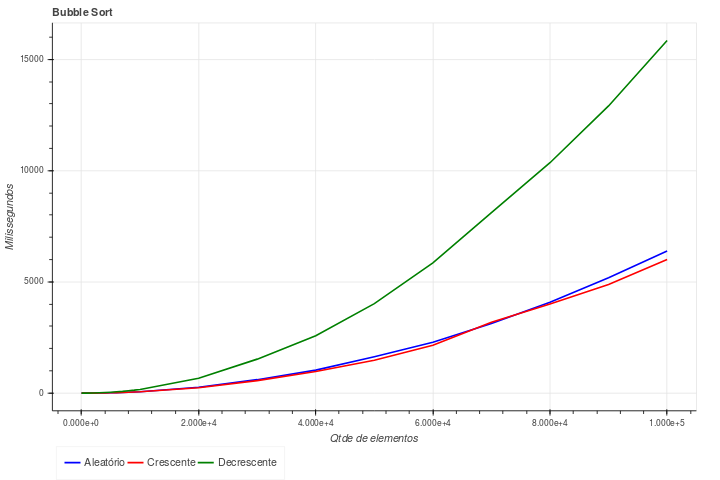
\includegraphics[scale=0.6]{img/algoritmos/bubble_sort.png}
	\caption{Bubble Sort, gráfico de resultados.}
	\label{graph-bubble}
\end{figure}

\subsection{Shell sort}
\begin{longtable}{|r|c|c|c|}
	\hline
	\csvreader[
		column count=5,
		no head,
		table head=\hline,
		late after line=\\\hline
	]{csvs/Shell_Sort.csv}{
		1=\n-elementos, 2=\aleatorio, 3=\crescente, 4=\decrescente
	}{ \n-elementos & \aleatorio & \crescente & \decrescente }
	\caption{Média de tempo do Shell Sort}
	\label{t-shell}
\end{longtable}

\begin{figure}[H]
	\centering
	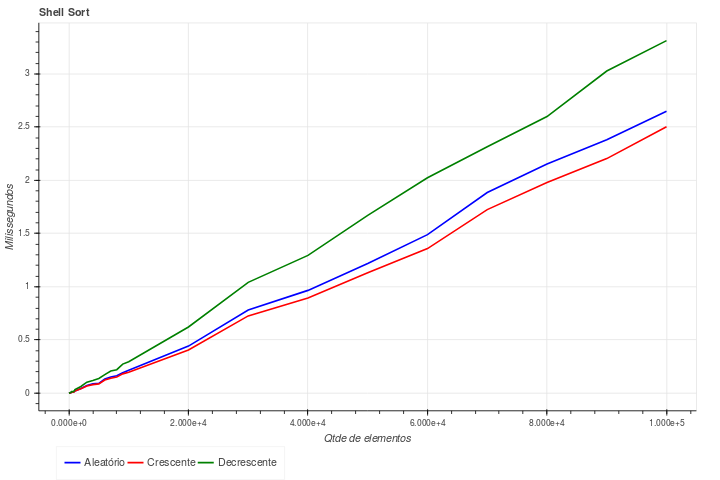
\includegraphics[scale=0.6]{img/algoritmos/shell_sort.png}
	\caption{Shell Sort, gráfico de resultados.}
	\label{graph-shell}
\end{figure}

\subsection{Quicksort}
\begin{longtable}{|r|c|c|c|}
	\hline
	\csvreader[
		column count=5,
		no head,
		table head=\hline,
		late after line=\\\hline
	]{csvs/Quicksort.csv}{
		1=\n-elementos, 2=\aleatorio, 3=\crescente, 4=\decrescente
	}{ \n-elementos & \aleatorio & \crescente & \decrescente }
	\caption{Média de tempo do Quicksort}
	\label{t-quick}
\end{longtable}

\begin{figure}[H]
	\centering
	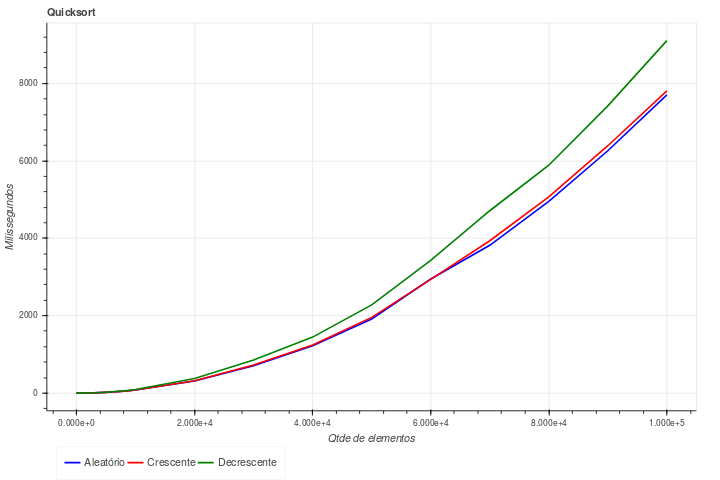
\includegraphics[scale=0.6]{img/algoritmos/quicksort.png}
	\caption{Quicksort, gráfico de resultados.}
	\label{graph-quicksort}
\end{figure}

\subsection{Merge sort}
\begin{longtable}{|r|c|c|c|}
	\hline
	\csvreader[
		column count=5,
		no head,
		table head=\hline,
		late after line=\\\hline
	]{csvs/Merge_Sort.csv}{
		1=\n-elementos, 2=\aleatorio, 3=\crescente, 4=\decrescente
	}{ \n-elementos & \aleatorio & \crescente & \decrescente }
	\caption{Média de tempo do Merge Sort}
	\label{t-merge}
\end{longtable}

\begin{figure}[H]
	\centering
	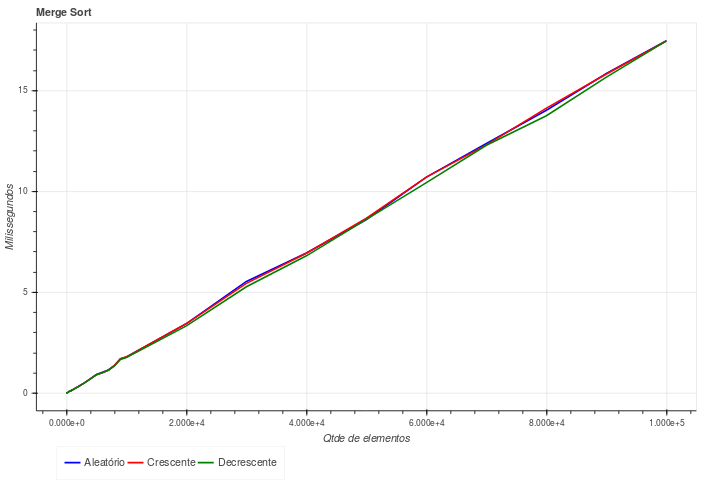
\includegraphics[scale=0.6]{img/algoritmos/merge_sort.png}
	\caption{Merge Sort, gráfico de resultados.}
	\label{graph-merge}
\end{figure}

\subsection{Radix sort (LSD)}
\begin{longtable}[c]{|r|c|c|c|}
	\hline
	\csvreader[
		column count=5,
		no head,
		table head=\hline,
		late after line=\\\hline
	]{csvs/Radix_sort_(LSD).csv}{
		1=\n-elementos, 2=\aleatorio, 3=\crescente, 4=\decrescente
	}{ \n-elementos & \aleatorio & \crescente & \decrescente }
	\caption{Média de tempo do Radix Sort (LSD)}
	\label{t-radix}
\end{longtable}

\begin{figure}[H]
	\centering
	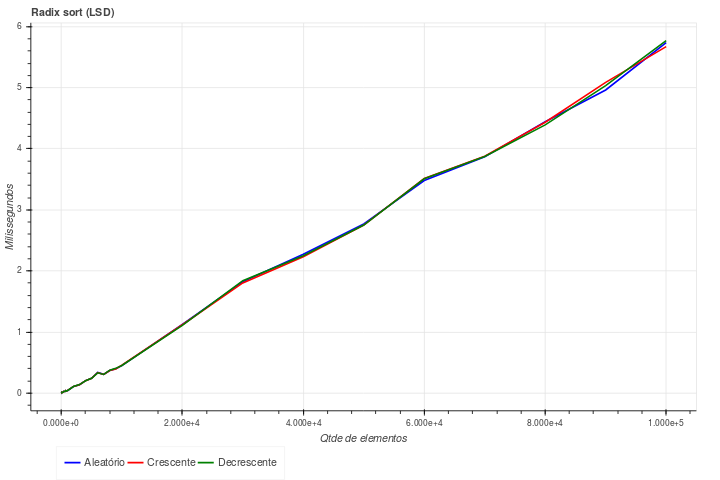
\includegraphics[scale=0.6]{img/algoritmos/radix.png}
	\caption{Radix sort (LSD), gráfico de resultados.}
	\label{graph-radix}
\end{figure}

\section{Resultados gerais}


\begin{figure}[H]
	\centering
	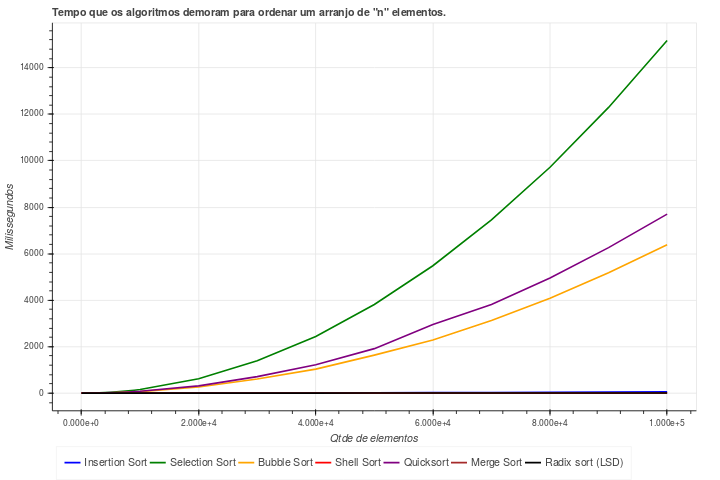
\includegraphics[scale=0.6]{img/graficos/aleatorios.png}
	\caption{Gráfico de resultados para arranjos com elementos aleatórios.}
	\label{graph-aleatorios}
\end{figure}

\begin{figure}[H]
	\centering
	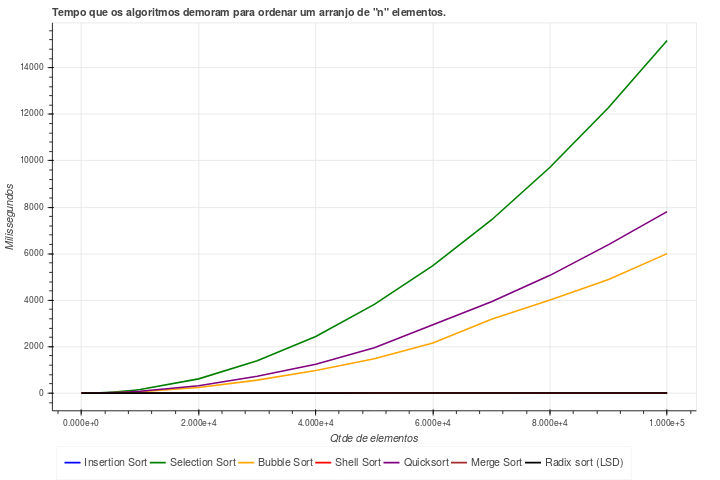
\includegraphics[scale=0.6]{img/graficos/crescentes.png}
	\caption{Gráfico de resultados para arranjos com elementos em ordem crescente.}
	\label{graph-crescentes}
\end{figure}

\begin{figure}[H]
	\centering
	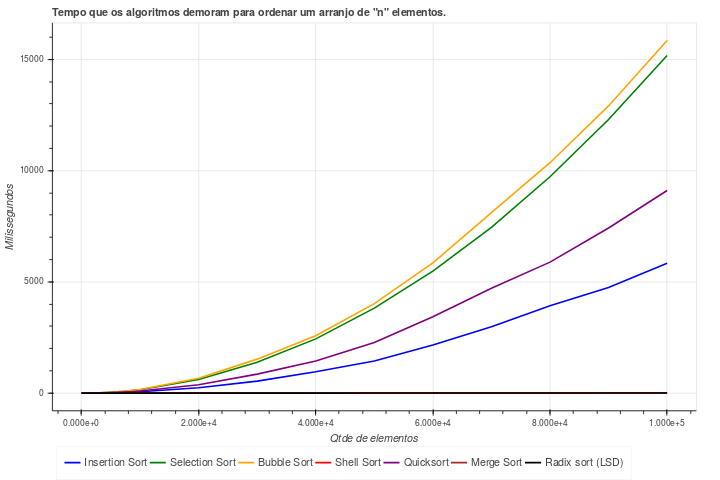
\includegraphics[scale=0.6]{img/graficos/decrescentes.png}
	\caption{Gráfico de resultados para arranjos com elementos em ordem decrescente.}
	\label{graph-decrescentes}
\end{figure}
\chapter{Discussão}
De maneira geral, podemos ver a clara diferença que faz escolher um algoritmo de ordenação ideal, sendo dos 7 analisados, apenas 3 bons o suficiente para uso com arranjos grandes. Pode-se também notar que a escolha do algoritmo não faz tanta diferença se considerarmos arranjos de apenas 100 elementos ou menores, como pode ser visto nos gráficos seguintes:

\begin{figure}[H]
	\centering
	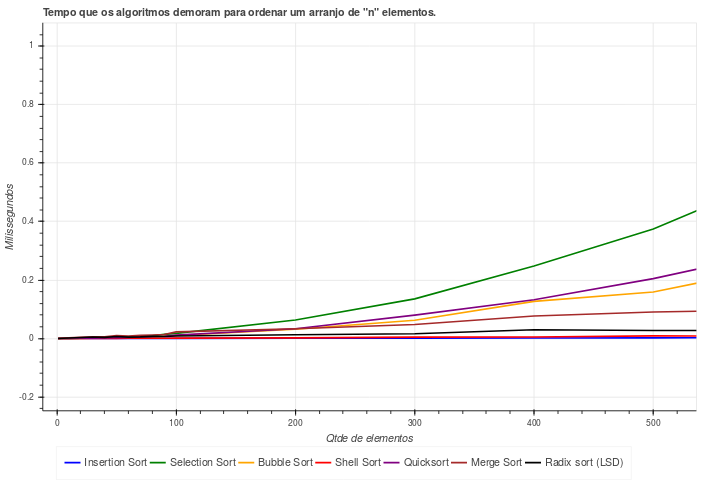
\includegraphics[scale=0.6]{img/igualdade/aleatorios.png}
	\caption{Gráfico de resultados para arranjos com os 100 primeiros elementos aleatórios.}
	\label{graph-aleatorio-comp}
\end{figure}

\begin{figure}[H]
	\centering
	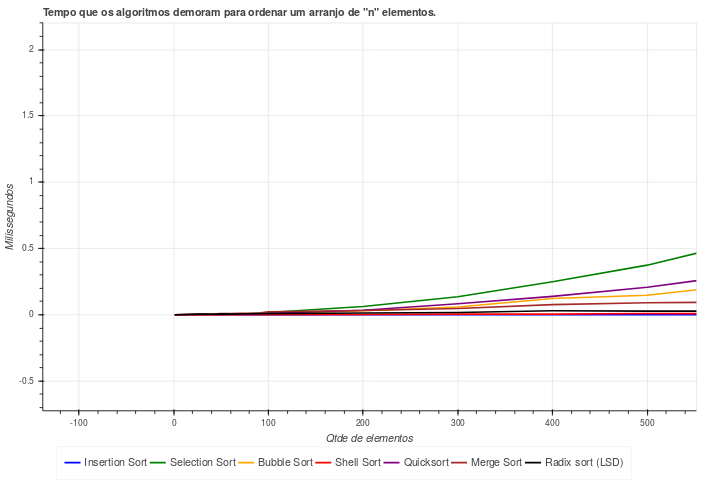
\includegraphics[scale=0.6]{img/igualdade/crescentes.png}
	\caption{Gráfico de resultados para arranjos com os 100 primeiros elementos em ordem crescente.}
	\label{graph-crescente-comp}
\end{figure}

\begin{figure}[H]
	\centering
	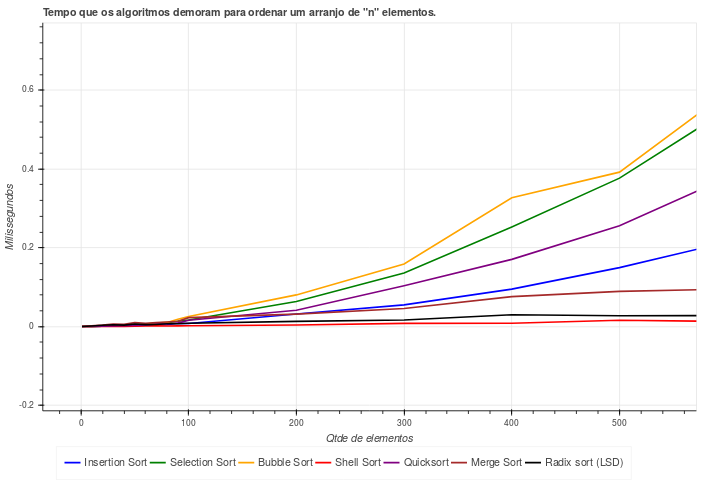
\includegraphics[scale=0.6]{img/igualdade/decrescentes.png}
	\caption{Gráfico de resultados para arranjos com os 100 primeiros elementos em ordem decrescente.}
	\label{graph-decrescente-comp}
\end{figure}

Dos 7, o algoritmo mais recomendado para uso é o \texttt{Shell sort}, pois no seu pior caso (ordem decrescente dos elementos) ele obteve uma média de $3.3127751999999986$ milissegundos, enquanto o segundo melhor algoritmo, \texttt{Radix sort (LSD)}, obteve $5.770450800000001$, pouco mais de dois milissegundos de diferença.

Mesmo sendo o segundo melhor algoritmo desse estudo, o \texttt{Radix sort (LSD)} mostrou-se ser muito superior a grande parte dos algoritmos de ordenação que utilizam comparação de chaves, visto que o \texttt{Radix} utiliza a decomposição das chaves.

Observando os valores dos algoritmos que utilizam recursão, \texttt{Quicksort} e \texttt{Merge sort}, podemos ver que o \texttt{Quick} é melhor se comparado ao \texttt{Merge} na ordenação dos arranjos de 100 elementos ou menores. Porém, o \texttt{Merge} mostrou-se ser bastante mais eficaz que o \texttt{Quick} a medida que a quantidade de elementos nos arranjos ia subindo, possuindo uma diferença entre seus piores casos de 9090 segundos.

Algo interessante a se notar, é a aproximação dos resultados quanto comparado os valores para arranjos aleatórios e arranjos crescentes, havendo uma diferença mais significante quanto comparado com os valores para arranjos decrescentes (piores casos).

\bibliography{bib/relatorio.bib}

\end{document}